
\item An infinitely long hollow conducting cylinder with inner radius \(R/2\) and outer radius \(R\) carries a uniform current density along its length. The magnitude of the magnetic field, \(|\vec{B}|\), as a function of the radial distance \(r\) from the axis is best represented by
\begin{tasks}(2)
    \task 
    \begin{center}
        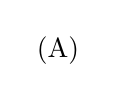
\begin{tikzpicture}
            \node at (0, 0) {(A)};
        \end{tikzpicture}
    \end{center}
    \task
    \begin{center}
        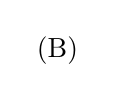
\begin{tikzpicture}
            \node at (0, 0) {(B)};
        \end{tikzpicture}
    \end{center}
    \task
    \begin{center}
        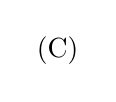
\begin{tikzpicture}
            \node at (0, 0) {(C)};
        \end{tikzpicture}
    \end{center}
    \task
    \begin{center}
        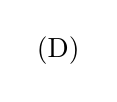
\begin{tikzpicture}
            \node at (0, 0) {(D)};
        \end{tikzpicture}
    \end{center}
\end{tasks}
